%----------------- CHAPTER 2 -------------------------------------------
%--------INTERFEROMETERS-----------------------------------------------
%% This is chapter two. Its a general motivation for using laser
%% interferometers and then a description of tricks used to extend
%% the sensitivity.
%% 
\chapter{Gravitational Wave Antennae}
\label{chap:IFO}

\begin{figure}[!h]
\centerline{\includegraphics[angle=0,width=6.5in]{Figures/Chap2/BeamTube2b.jpg}}
\end{figure}
\clearpage

A gravitational wave detector must be a transducer for turning space-time strain 
into a recordable signal (current, voltage, etc.). Since the coupling of gravitational
radiation to matter is very weak, much effort has been devoted to constructing
very efficient transducers. This chapter briefly motivates the optical
configuration used in LIGO and then describes the gravitational wave signal readout path.



% --------------------------------------------------------------------------------------
\section{Resonant Mass Detectors (Bars)}

Four decades after they had been predicted by theory, Joseph Weber reported 
on a method for detecting gravitational waves using a large aluminum bar\cite{Weber:1960}. 
The idea was that a passing gravitational wave
would induce a strain on the bar, exciting the bar's resonant modes. 
For reasons detailed elsewhere\cite{Levine:Bar,Tyson:Bar}, the
community was never able to verify Weber's subsequent claims of 
detection\cite{Weber:1969}
although various theories\cite{Misner:beaming,Hawking:Bursts} were developed 
to explain the enormous apparent flux of gravitational wave energy.

Following Weber's pioneering work, various international efforts 
to increase the sensitivity of resonant mass detectors began.
Today's best
bars are seismically isolated and cryogenically cooled to reduce the
natural vibration of the bar, and the use of SQUIDs to readout the signals
has dramatically increased the sensitivity\cite{Bars}.

There are also highly ambitious proposals\cite{Spheres} for more
sophisticated geometries (spheres, dodecahedrons, etc.) designed to improve the 
bandwidth and directional sensitivity of the resonant mass detectors.



% --------------------------------------------------------------------------------------
\section{Laser Interferometers}

The idea of measuring the geodesic deviation with pulses of light was
first published by Pirani in 1956~\cite{Pirani:GR}.
The first prototype interferometer for gravitational wave detection was built
in the early 70s in Malibu~\cite{Forward:Interferometer}. Almost all of the
limiting noise sources which we contend with today were laid out by R. Weiss 
in a study done at MIT~\cite{Rai:QPR}.

Many different interferometer configurations are sensitive to gravitational waves
(see \cite{Mizuno:Thesis} and references therein).
This section will describe briefly each of the sub components of the
power-recycled, Fabry-Perot Michelson interferometer configuration used in
LIGO.

All of the kilometer-scale interferometers in the world are planned to
be variants of the power-recycled Michelson scheme. Alternative 
interferometer configurations, such as Sagnac interferometers \cite{Rai:NSF,Byer:Sagnac}
and resonant recycling \cite{Drever:Houches}, have also been explored.


\subsection{The Michelson Interferometer}

The core of the LIGO interferometer is a Simple Michelson (SM) interferometer. 
The SM consists of a light source (a laser in our case) illuminating a 50/50 beamsplitter.
The transmitted and reflected beams from the beamsplitter travel perpendicular
paths, are reflected from two end mirrors, and then recombine at the beamsplitter.

\begin{figure}[!h]
\centerline{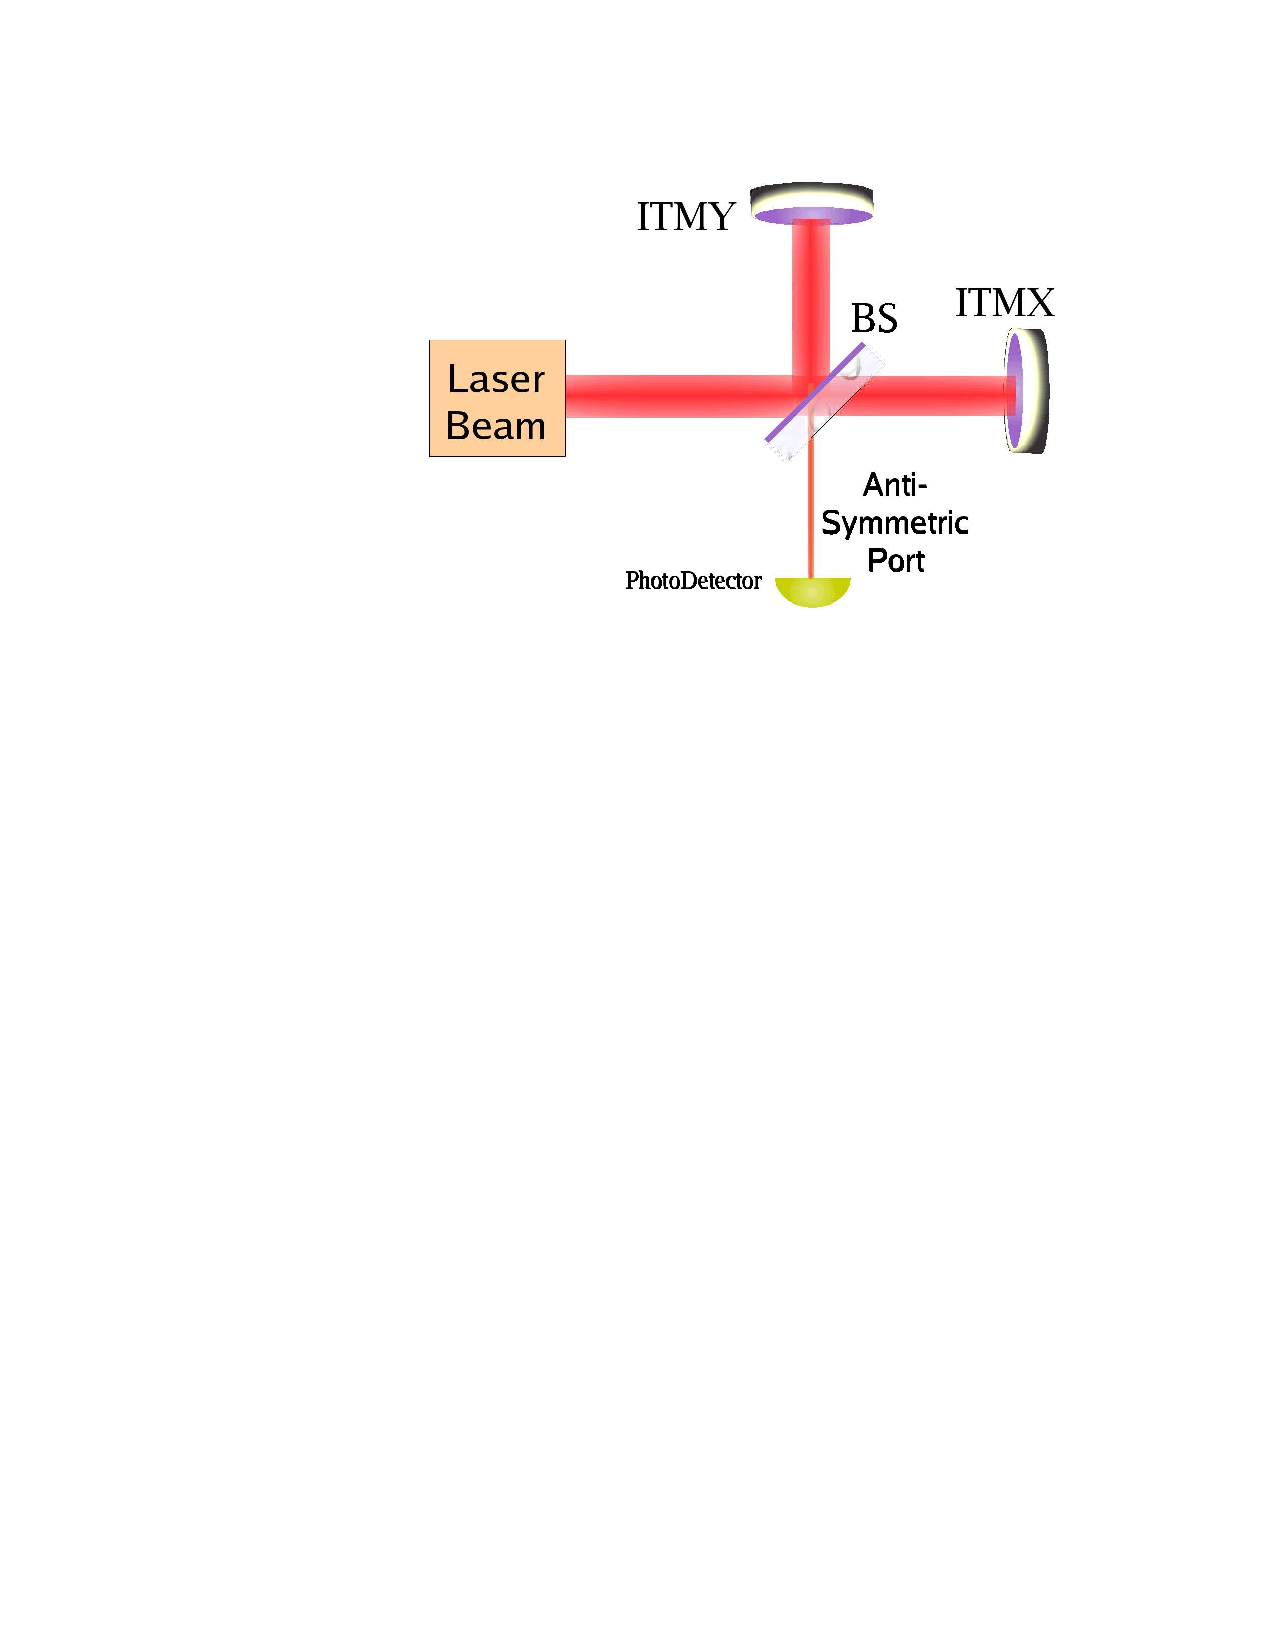
\includegraphics[angle=0,height=3.5in]{Figures/Chap2/Michelson.pdf}}
\caption[Michelson Diagram]{A basic Michelson type interferometer. The field from the
         laser comes in from the symmetric side of the beamsplitter. The light from the
         two arms interferes destructively at the AS port.}
\label{fig:Michelson}
\end{figure}
The resulting electric field at the Anti-Symmetric (AS) port is a function of
the effective optical path difference for the beams in the two arms. 

\begin{equation}
E_{AS} = E_{in} (r_{ex} t_{bs} r_{bs} e^{i 2 \phi_x} - r_{ey} t_{bs} r_{bs} e^{i 2 \phi_y})
\label{eq:SM}
\end{equation}
where  $\phi_x$ \& $\phi_y$ are the phases accumulated by the light in a single trip
down each arm (i.e. $\phi_{rt} = 2 \phi_x$) and $t_{bs}$ \& $r_{bs}$ are the field 
transmission and reflection, respectively,of the beamsplitter.

For an optical interferometer, the electromagnetic radiation is at frequencies
greater than 10$^5$ GHz. This is too high a frequency to detect with present day
technologies. Instead, detectors are used which are sensitive to the envelope of
the field. For visible and near infrared wavelengths, one such detector is the 
photodiode, which emits a current. This photo-electron current is proportional 
to the average photon flux, or power, on the detector.

If we ask what the power at the AS port is for the case in which the end mirrors
have identical reflectivities ($r_{ex} = r_{ey} = r_e$), we get from 
Equation~\ref{eq:SM} that:

$P_{AS} = E^{*}E = 4 |E_{in}|^2(r_e t_{bs} r_{bs})^2 \sin{(\phi_{-})}^2$
where $\phi_{-} = \phi_y - \phi_x$. 
The phase sensitivity is $\frac{d \, P}{d \, \phi_{-}}$. In the simple case where
$r_e = 1$ and $r_{bs} \times t_{bs} = 1/2$, we get

\begin{equation}
\frac{d \, P}{d \, \phi_{-}} = 2 P_{bs} sin(\phi_-) cos(\phi_-) 
\end{equation}
where $P_{bs} \equiv |E_{in}|^2$. The measured power fluctuations due to 
shot noise (more in Section~\ref{sec:ShotNoise}) are:

\begin{equation}
\delta P_{shot} = \sqrt{\frac{2 h c}{\lambda} P_{bs} \sin{\phi_-}^2}
\end{equation}
and so the equivalent \emph{phase noise} is just the ratio:

\begin{equation}
 \begin{aligned}
  \frac{\delta \phi_-}{\sqrt{\mbox{Hz}}} 
         &= \sqrt{\frac{1}{2} \frac{h c}{\lambda} 
            \frac{1}{P_{bs}} \frac{1}{\cos{\phi_-}^2}} \\
         &\simeq 3 \times 10^{-11} \left(\frac{100 \mbox{W}}{P_{bs}}\right)^{1/2}
            \frac{\mbox{radians}}{\sqrt{\mbox{Hz}}}
 \end{aligned}
\label{eq:PhaseNoise}
\end{equation}
where the estimate is for the LIGO laser wavelength of 1064 nm and the phase
offset in the Michelson is small.


\subsection{Fabry-Perot Resonators}

Looking at Equation~\ref{eq:h}, a clear way to increase the strain sensitivity is 
to make very long arms in a
Michelson interferometer. For terrestrial interferometers, the arm length
is limited by technical annoyances such as cost and the availability of a large,
quiet piece of land. A technique which is almost as good as having long
arms is to bounce the beam multiple times in each arm.

This type of delay line~\cite{Herriot}, was proposed \cite{Rai:QPR} as a way 
of increasing the signal gain of the interferometers. Experiments with
this topology \cite{David:Garching} uncovered technical problems due to
scattered light which make this idea impractical, although it has been
pointed out that operating the interferometer with white light is a possibility.

An alternative to this method is to overlap the multiple reflections on 
the same spot on the mirror \cite{Drever:Houches}. By making the
input mirror of the arm into a partial transmitter and adjusting the separation
between the mirrors carefully, the input mirror and end mirror can be made into a
Fabry-Perot resonator \cite{FabryPerot}. The disadvantage with this technique
compared to the delay lines is that the cavity must be operated near resonance
to achieve the high power buildup and resultant phase shift gain which the
delay line has at any operating point. This resonant operation is achieved through
the use of feedback control of the cavity length.




\subsection{Power Recycling}

In the Michelson shown in Figure~\ref{fig:Michelson}, the light returning from
the two arms interferes constructively in the direction heading back to the laser.
Effectively then, the Michelson interferometer looks like a highly reflecting
mirror, when it is adjusted for maximum darkness at the anti-symmetric port.
This reflected light would be dumped somewhere and not contribute to the signal
gain of the interferometer. 

\begin{figure}[!h]
\centerline{\includegraphics[angle=0,height=3.5in]{Figures/Chap2/PRM.pdf}}
\caption[PRM Diagram]{A partially transmitting mirror on the symmetric side
         of a Michelson makes power-recycled Michelson.}
\label{fig:PRM}
\end{figure}
By placing a partially transmitting mirror between the laser and the beamsplitter,
as shown in Figure~\ref{fig:PRM}, one can send this light back into 
the interferometer. The Michelson part of the
interferometer acts on the incoming light like a high reflectance mirror and
can potentially form a high finesse, Fabry-Perot cavity with this new mirror.
This technique is called power 
recycling~\cite{Peter:Thesis,Schilling:Recycling,Drever:Houches} 
and the added mirror is the power recycling mirror (RM).

The following are some further qualitative comments about power recycling which
are more quantitatively described in the following chapters:

\begin{itemize}

\item The RM transmission is chosen to equal as closely as possible, all of the
      other losses experienced by the carrier field in the interferometer (see
      Appendix~\ref{app:optics} for details on losses). 
      The matching is done so that all of the carrier light is coupled into
      the interferometer. The power gain achieved through power recycling is
      $\sim$40-50 in LIGO.

\item The increased power available in the Michelson increases the shot noise 
      limited \emph{phase} sensitivity of the Michelson 
      by putting more light on the Beamsplitter (see Equation~\ref{eq:PhaseNoise}. 

\item The resonance linewidth of the big coupled cavity, formed by the power recycling
      mirror and the arm cavities, is much narrower than the linewidth of the
      arm cavity alone. The coupled cavity pole, $f_{cc}$, is equal to
      $f_c / \mathcal{F}_{RC}$, the arm cavity pole frequency divided by the 
      Finesse of the recycling cavity.
      The beauty of this narrowing is that the \emph{carrier} field which is in the 
      interferometer has been passively filtered by a $\sim$1 Hz low pass filter on 
      top of all of the active stabilization. In this way, we would be able to
      achieve another factor of 100 suppression of the technical laser noise.

\item Power recycling does not reduce the bandwidth of the gravitational wave readout
      at the anti-symmetric port, since differential signals produced in the
      arms \emph{are not recycled}.

\end{itemize}






